% FIG ch02-06 NMC final overlay (Chinese) — requires codex base image
\begin{tikzpicture}
  \node[anchor=south west, inner sep=0] (img) at (0,0)
    {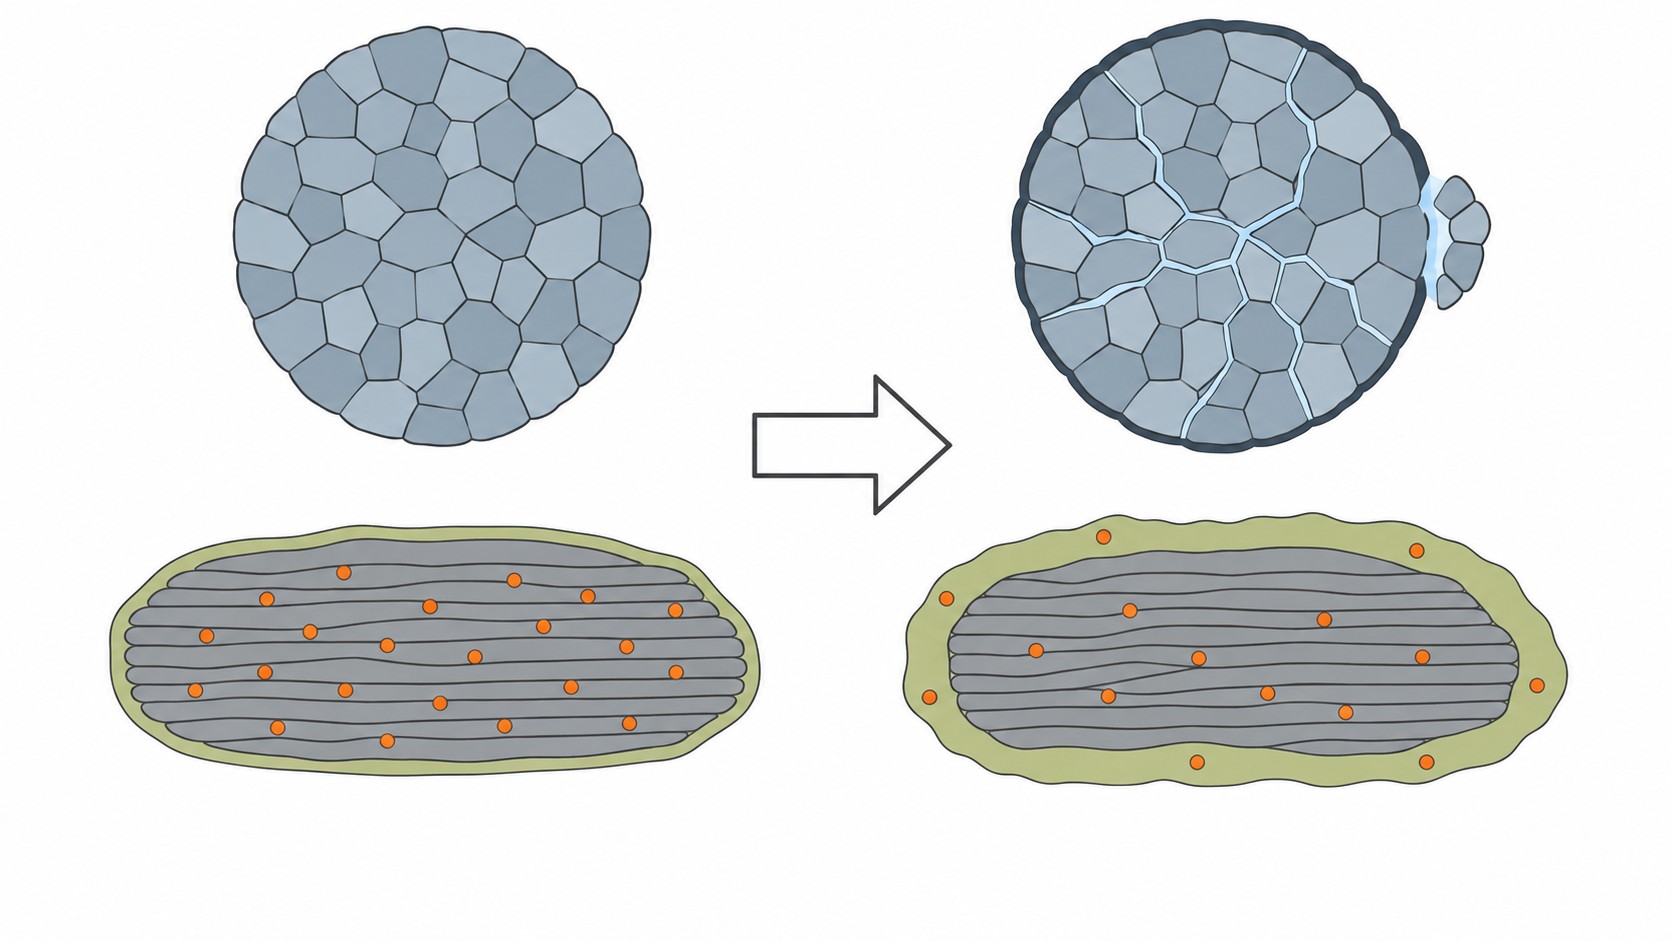
\includegraphics[width=\linewidth]{figures/ch02/ch02-06-nmc-v3-base.png}};
  \begin{scope}[x={(img.south east)}, y={(img.north west)},
    font=\sffamily\fontsize{7}{8}\selectfont]
    \node[font=\bfseries] at (0.25, 0.96) {新鲜};
    \node[font=\bfseries] at (0.75, 0.96) {循环后};
    \node[align=center, anchor=west] at (0.04, 0.70) {NMC\\正极\\二次颗粒};
    \node[anchor=west] at (0.04, 0.30) {石墨负极};
    \node at (0.50, 0.58) {循环};
    \node[anchor=west] at (0.14, 0.86) {初级晶粒};
    \draw[BookInk!40, thin] (0.14, 0.84) -- (0.18, 0.82);
    \node[anchor=west] at (0.66, 0.88) {沿晶微裂纹（电解液渗入）};
    \draw[BookInk!40, thin] (0.66, 0.86) -- (0.58, 0.84);
    \node[draw=BookInk, line width=0.4pt, fill=white, fill opacity=0.85, text opacity=1,
      align=left, inner sep=2pt, anchor=west] at (0.90, 0.80)
      {表面重构层\\→ 阻抗升高};
    \node[draw=BookInk, line width=0.4pt, fill=white, fill opacity=0.85, text opacity=1,
      align=left, inner sep=2pt, anchor=west] at (0.90, 0.62)
      {碎块失去接触\\→ 活性材料损失};
    \node[draw=BookInk, line width=0.4pt, dashed, fill=white, fill opacity=0.85, text opacity=1,
      align=left, inner sep=2pt, anchor=west] at (0.66, 0.52)
      {裂纹新表面副反应\\→ 阻抗升高（推测）};
    \node[anchor=west] at (0.12, 0.18) {SEI};
    \draw[BookInk!40, thin] (0.12, 0.20) -- (0.16, 0.22);
    \node[draw=BookInk, line width=0.4pt, fill=white, fill opacity=0.85, text opacity=1,
      align=left, inner sep=2pt, anchor=west] at (0.86, 0.22)
      {SEI 增厚\\→ 可循环锂减少};
  \end{scope}
  \begin{scope}[x={(img.south east)}, y={(img.north west)},
    font=\sffamily\scriptsize]
    \node[align=center] at (0.50, 0.05) {%
      图例：实线框 = 文献确立；虚线框 = 作者推测；橙点 = 锂（示意）};
  \end{scope}
\end{tikzpicture}
